\chapter{Appendix I: Day/Night Zoning}
\label{appendix:i}


\begin{figure*}[ht]
  \centering
  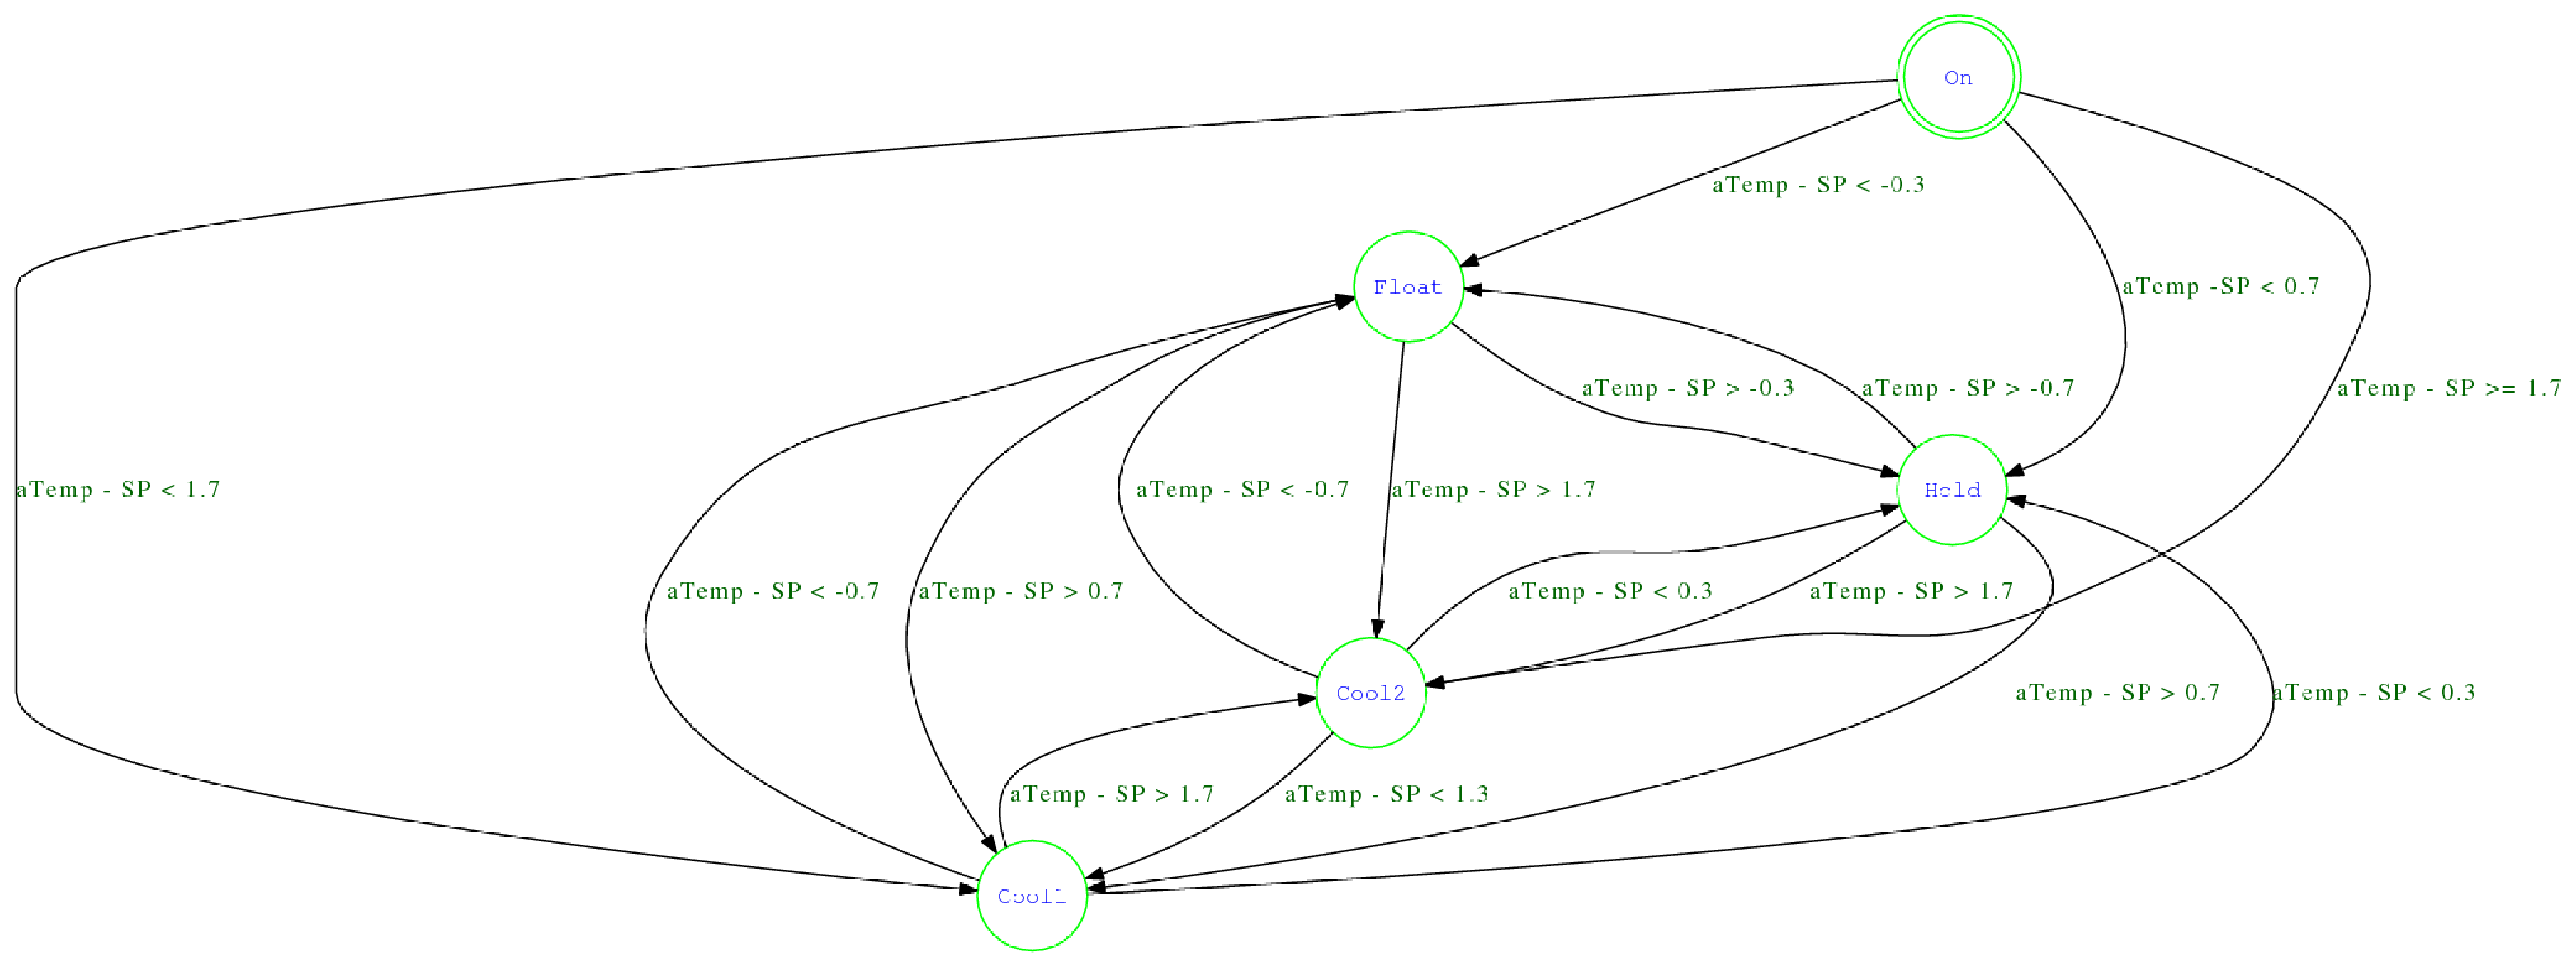
\includegraphics[width=1.0\columnwidth]{fig/fsm.eps}
  \caption[Finite State Machine of Day/Night Zoning Controller]{The
  zoning controller attempts to maintain the average temperature of the active
  zone (aTemp) at the desired setpoint (SP) by transitioning the system between
  five states.}
  \label{fig:stateMachine}
\end{figure*}


\begin{figure}
  \begin{macrolab}
RTS = RunTimeSystem();
weatherdirect = RTS.getMotes('type', 'weatherdirect');
tempSensors = SensorVector(weatherdirect, 'temperature');
x10 = RTS.getMotes('type', 'X10');
motionSensors = SensorVector(x10, 'motion');
zones = uint8({[3 4 5], [1 2 6 7]}); % Day/Night zones
motionSensorIDs = uint8({[8 1 9], [2 6], [10 5], [4], [7 11], [12 14], [3 15]})
tempSensorIDs = uint8({[1 3], [2], [6 7], [4 9 11], [12 13], [5 14], [8 10]}) 
nightStart = [0 0 0 2 0 0];
nightEnd = [0 0 0 7 0 0];
curState = 'On'
every(60000)
  mode = RTS.dbRead('zoning', 'mode', 'latest')
  motionVals = motionSensors.sense();
  tempVals =  tempSensors.sense();
  curTime = clock;
  curNightStart = nightStart;
  curNightStart(1:3) = curNightStart(1:3) + curTime(1:3);
  curNightEnd = nightEnd;
  curNightEnd(1:3) = curNightEnd(1:3) + curTime(1:3);
  curZone = {}
  if datenum(curTime) <= datenum(curNightStart) && datenum(curTime) > datenum(curNightEnd)  
    curZone = zones{1}
  else
    curZone = zones{2};
  end
  curZoneMotion = []
  curZoneTemps = []
  for room = curZone
    curZoneMotion = [curZoneMotion motionVals(motionSensorIDs{room})]
    curZoneTemps = [curZoneTemps tempVals(tempSensorIDs{room})]
  end
  if sum(curZoneMotion) > length(curZoneMotion) / 2
    occupied = true;
    SP = dbRead('zoning', 'setpoint', 'latest');
  else
    occupied = false;
    SP = dbRead('zoning', 'setback', 'latest')
  aTemp = mean(curZoneTemps);
  if mode == 'heat'
    deltaTemp = SP - aTemp;
  else
    deltaTemp = aTemp - SP;

  curState = getNextState(curState, deltaTemp);

  hvacActuate(mode, curState, curZone)
end
  \end{macrolab}
  \smallskip
  \hrule width 1\columnwidth
  \caption{MacroLab implementation of day/night zoning.}
  \label{code:cs1}
\end{figure}

\begin{figure}
  \begin{macrolab}
function getNextState(curState, deltaTemp)
  if curState == 'On'
    if deltaTemp < -0.3
      curState = '-1' % float
    elif deltaTemp < 0.7
      curState = '0' % hold
    elif deltaTemp < 1.7
      curState = '1' % heat/cool 1
    elif deltaTemp >= 1.7
      curState = 2 % heat/cool 2
  elif state == '-1'
    if deltaTemp > -0.3
      curState = '0'
    elif deltaTemp > 0.7
      curState = '1'
    elif deltaTemp > 1.7
      curState = '2' 
  elif state == '1'
    if deltaTemp < -0.7
      curState = '-1'
    elif deltaTemp < 0.3
      curState = '0'
    elif deltaTemp > 1.7
      curState = '2'
end
  \end{macrolab}
  \smallskip
  \hrule width 1\columnwidth
  \caption{MacroLab function to calculate transition in hysteresis state
  machine.}
  \label{code:getNextState}
\end{figure}
